\documentclass[11pt,letterpaper]{article}

% ─── Packages ───────────────────────────────────────────────────
\usepackage[margin=1in]{geometry}
\usepackage[utf8]{inputenc}
\usepackage[T1]{fontenc}
\usepackage{amsmath,amssymb,amsthm}
\usepackage{mathtools}
\usepackage{thmtools}
\usepackage{tikz}
\usetikzlibrary{arrows.meta,positioning,calc,decorations.markings,patterns,shapes.geometric}
\usepackage{pgfplots}
\pgfplotsset{compat=1.18}
\usepackage{algorithmic}
\usepackage{graphicx}
\usepackage{textcomp}
\usepackage{xcolor}
\usepackage{hyperref}
\usepackage{cleveref}
\usepackage{booktabs}
\usepackage{microtype}
\usepackage{enumitem}
\usepackage{authblk}

% ─── Theorem Environments (thmtools for cleveref integration) ───
\declaretheorem[name=Theorem,numberwithin=section]{theorem}
\declaretheorem[name=Lemma,sibling=theorem]{lemma}
\declaretheorem[name=Proposition,sibling=theorem]{proposition}
\declaretheorem[name=Corollary,sibling=theorem]{corollary}
\declaretheorem[name=Definition,sibling=theorem,style=definition]{definition}
\declaretheorem[name=Remark,sibling=theorem,style=definition]{remark}
\declaretheorem[name=Example,sibling=theorem,style=definition]{example}

% ─── Notation shortcuts ────────────────────────────────────────
\newcommand{\R}{\mathbb{R}}
\newcommand{\N}{\mathbb{N}}
\newcommand{\kJ}{\kappa_J}
\newcommand{\eps}{\varepsilon}
\newcommand{\topomass}{M}
\newcommand{\Excit}{E}
\newcommand{\Mod}{\Phi}
\newcommand{\Topo}{\Omega}
\newcommand{\Info}{I}
\newcommand{\Ent}{H}
\newcommand{\meangrad}{\bar{\kappa}'_J}

\hypersetup{
  colorlinks=true,
  linkcolor=blue!60!black,
  citecolor=green!40!black,
  urlcolor=blue!60!black
}

% ─── Document ───────────────────────────────────────────────────
\begin{document}

\title{Excitability Topology and the Obsolescence of Price:\\
Currency as Modulation, Coherence as Market}

\author{Larsen James Close}
\affil{Independent Researcher}

\date{February 2026}

\maketitle

% ════════════════════════════════════════════════════════════════
% ABSTRACT
% ════════════════════════════════════════════════════════════════
\begin{abstract}
Currency exists because agents cannot directly observe each other's readiness to coordinate.
Price signals compress this hidden structure---an agent's \emph{excitability topology}---into transferable scalars.
We show that a system making excitability topology directly legible renders price redundant: under complete topological legibility, the mutual information between price and excitability vanishes (with a continuous bound for partial legibility).
We formalize excitability topology over interaction graphs, define currency as a modulation operator on that topology, and map the framework onto the Disentangle protocol's Jaccard-based Ollivier-Ricci curvature.
The curvature derivative $\partial\kJ/\partial d$ measures the rate of coordination formation---a structural analog of dopaminergic prediction-error signaling.
Agents interpreting this derivative as ``return on investment'' and agents interpreting it as ``where is genuine information being created'' produce identical graph dynamics, making the transition from price-mediated to topology-mediated coordination structurally gradual and ideology-independent.
\end{abstract}

\medskip\noindent\textbf{Keywords:} excitability topology, curvature, Ollivier-Ricci, consensus, resource allocation, dopamine, price theory, information theory

% ════════════════════════════════════════════════════════════════
\section{Introduction}\label{sec:intro}
% ════════════════════════════════════════════════════════════════

The standard account of currency identifies three functions: store of value, medium of exchange, and unit of account.
These are descriptions of \emph{what} currency does.
They do not explain \emph{why} it does it---what information-processing problem currency solves that no other mechanism addresses.

We propose a mechanistic account.
Currency is a technology for \emph{remotely modulating excitability topologies} across agents whose internal states are opaque.
An agent's excitability topology is the structure of its readiness to respond to coordination signals from other agents.
When this structure is invisible---when you cannot read whether another agent is ready, willing, and capable of coordinating on a particular task---you require a \emph{transferable modulation token} to shift their readiness from outside.
That token is currency.

This framing recasts familiar monetary phenomena.
A wage is a technique for remotely modulating an employee's action-readiness toward specific tasks.
A price is a signal encoding the excitability gradient of a good's production network.
Debt is a temporal displacement of excitability modulation.
A derivative is meta-modulation: a token whose value derives from anticipated future shifts in excitability landscapes.

The standard functions follow from this mechanism:
\emph{store of value} is stored capacity to modulate others' action-readiness;
\emph{medium of exchange} is the transferability of modulation tokens between agents;
\emph{unit of account} is the quantization of modulation capacity into comparable scalar units.

The critical observation is that currency's \emph{necessity} depends on a precondition: the opacity of excitability topologies.
If excitability topology becomes directly legible---if a system can measure, in real time, which agents are coordinating well and where coordination is actively forming---then the proxy becomes redundant.
The information that price signals encode is already available in the topology (cf.~\cite{hayek1945}, which identifies price as the indispensable distributed-knowledge channel; we argue the precondition dissolves under legibility).

This paper formalizes and demonstrates this claim.
We draw on the Disentangle protocol~\cite{close2026}, which implements Topological Mass Consensus using Jaccard-based Ollivier-Ricci curvature~\cite{ollivier2009,pal2017} over a transaction DAG.
In that protocol, curvature $\kJ(u,v)$ measures the structural quality of the relationship between agents $u$ and $v$, and the curvature derivative $\partial\kJ/\partial d$ measures the \emph{rate} at which coordination quality is changing.
We show that these measurements constitute a direct reading of the excitability topology, eliminating the information-theoretic need for price.

\subsection{Contributions}

\begin{enumerate}[label=(\alph*)]
  \item A formal framework defining excitability topology over interaction graphs and currency as a modulation operator on that topology (\S\ref{sec:framework}).
  \item An information-theoretic theorem establishing conditions under which price signals become redundant (\S\ref{sec:redundancy}).
  \item A mapping from Disentangle protocol primitives to the excitability framework, identifying the curvature derivative as a dopaminergic market signal (\S\ref{sec:gradient}).
  \item A structural (not ideological) transition path from price-mediated to topology-mediated coordination, where pre-shift and post-shift agents produce identical graph dynamics (\S\ref{sec:transition}).
\end{enumerate}

\subsection{Scope and Caveats}

The claim is information-theoretic, not moral.
Price signals are useful under opacity conditions.
They become unnecessary under legibility conditions.
This is value-neutral: a flashlight does not render darkness ``bad''; it renders it navigable without stumbling.
Nothing in this paper advocates abolishing currency by fiat or asserts that price-mediated coordination is defective.
We argue only that a system providing sufficient topological legibility makes price a redundant encoding.

% ════════════════════════════════════════════════════════════════
\section{Background}\label{sec:background}
% ════════════════════════════════════════════════════════════════

\subsection{Dopamine as Excitability Modulator}\label{sec:dopamine}

The role of dopamine in neural computation has been substantially revised since Schultz's landmark finding that midbrain dopamine neurons encode \emph{prediction errors}, not reward~\cite{schultz1997}.
Dopamine modulates the firing thresholds of downstream circuits, altering which neural populations are ready to activate in response to input.
This creates an \emph{attention topology}: the pattern of relative excitability across neural circuits at a given moment.

Three properties of dopaminergic modulation are relevant to our argument:

\begin{enumerate}
  \item \textbf{Rate-of-change encoding.} Dopamine signals encode the \emph{derivative} of prediction quality, not its level. A consistently rewarding environment produces baseline dopamine, not elevated dopamine. The signal marks \emph{change}~\cite{schultz1997}.

  \item \textbf{Topological modulation.} Dopamine does not activate specific circuits; it modulates the \emph{landscape} of activation readiness. Which circuits fire depends on the interaction between the current dopamine-modulated topology and incoming sensory input~\cite{friston2017}.

  \item \textbf{Temporal integration.} Long-term potentiation (LTP) accumulates excitability history. Circuits that have been repeatedly brought to readiness by dopaminergic signals become structurally easier to activate---a form of topological memory~\cite{schultz1997}.
\end{enumerate}

\subsection{Currency as Externalized Dopamine}\label{sec:currency-dopamine}

We propose that currency performs, across a multi-agent network, the same function that dopamine performs within a single nervous system: it modulates the excitability topology of the network.

Consider the historical progression:
\begin{itemize}
  \item \textbf{Barter}: direct bilateral excitability modulation. Agent $A$ must find agent $B$ whose excitability topology is already aligned (the ``double coincidence of wants'').
  \item \textbf{Commodity money}: generalized modulation tokens. The token shifts any agent's action-readiness because it can be re-transferred~\cite{graeber2011}.
  \item \textbf{Credit}: temporal excitability modulation. The modulation occurs now; the reciprocal shift is deferred.
  \item \textbf{Derivatives}: meta-modulation. The token's modulation capacity depends on anticipated future shifts in excitability landscapes.
\end{itemize}

The critical structural feature is that \emph{currency works because internal states are unreadable}.
If agent $A$ could directly observe agent $B$'s excitability topology---which tasks $B$ is ready to coordinate on, how reliably $B$ follows through, what $B$'s coordination history looks like---then $A$ would not need a transferable token to assess or modulate $B$'s readiness.
The token is an \emph{opacity workaround}.

Legal tender enforcement is the backstop: when the modulation token fails to shift an agent's action-readiness (the agent refuses to coordinate despite payment), the legal system compels compliance.
This is external enforcement of failed excitability modulation.

\subsection{Topology-Based Consensus}\label{sec:topo-consensus}

The Disentangle protocol~\cite{close2026} implements consensus through geometric measurement of a transaction DAG rather than through economic incentives or computational work.
We summarize the elements relevant to this paper.

\begin{definition}[Jaccard Curvature~\cite{close2026,pal2017}]\label{def:jaccard}
For vertices $u,v$ connected by an edge in graph $G$, the Jaccard curvature is
\begin{equation}\label{eq:jaccard}
  \kJ(u,v) = 2 \cdot J\bigl(N(u), N(v)\bigr) - 1
\end{equation}
where $J(A,B) = |A \cap B| / |A \cup B|$ is the Jaccard index and $N(\cdot)$ denotes the neighbor set.
\end{definition}

\begin{definition}[Topological Mass~\cite{close2026}]\label{def:topmass}
For a transaction $t$ with confirmation window $W(t,\tau)$,
\begin{equation}\label{eq:topmass}
  \topomass(t) = \Bigl(\sum_{d \in W(t,\tau)} w(t,d) \cdot (1 + \log(1+r_d))\Bigr) \cdot D(t)
\end{equation}
where $w(t,d)$ is the curvature-weighted max-path weight, $r_d$ is verified reputation, and $D(t)$ is the diversity score.
\end{definition}

Topological mass is non-transferable, non-purchasable, and decays without ongoing participation~\cite{close2026}.
These properties---which are unusual for a value measure in distributed systems---follow directly from the fact that mass is a structural property of the graph, not a token held by a node.

The protocol further defines a \emph{CoherenceMinimum}: a threshold curvature below which an agent's participation is throttled.
This functions as an excitability gate: agents whose coordination quality falls below the threshold have reduced influence, analogous to a firing threshold in neural circuits.

% ════════════════════════════════════════════════════════════════
\section{Formal Framework}\label{sec:framework}
% ════════════════════════════════════════════════════════════════

\subsection{Excitability Topology}\label{sec:excit-topo}

\begin{definition}[Excitability Function]\label{def:excit}
Let $\mathcal{A}$ be a finite set of agents and $G = (\mathcal{A}, \mathcal{E})$ an interaction graph. An \emph{excitability function} is a map
\begin{equation}
  \Excit : \mathcal{A} \times \mathcal{A} \to [0, 1]
\end{equation}
where $\Excit(i,j)$ denotes the readiness of agent $i$ to respond to a coordination signal from agent $j$.
\end{definition}

The excitability function induces a topology on $\mathcal{A}$: subsets of agents with high mutual excitability form clusters; gradients in excitability define natural boundaries between coordination domains.

\begin{definition}[Excitability Topology]\label{def:excit-topo}
The \emph{excitability topology} $\Topo_\Excit$ on $(\mathcal{A}, \mathcal{E})$ is the weighted graph where each edge $(i,j) \in \mathcal{E}$ carries weight $\Excit(i,j) \cdot \Excit(j,i)$, representing mutual coordination readiness.
\end{definition}

\begin{definition}[Self-Governed vs.\ Externally Modulable Excitability]\label{def:self-gov}
Agent $i$'s excitability is \emph{self-governed} if $\Excit(i,j)$ is determined solely by $i$'s internal state and the history of $(i,j)$ interactions.
Agent $i$'s excitability is \emph{externally modulable} if there exists a modulation operator $\Mod$ such that $\Excit(i,j)$ can be shifted by token injection from a third party $k \neq j$.
\end{definition}

The distinction is structural: in a self-governed regime, excitability reflects genuine coordination capacity; in an externally modulable regime, it reflects the distribution of modulation tokens.

\subsection{Currency as Modulation Operator}\label{sec:currency-operator}

\begin{definition}[Modulation Operator]\label{def:mod-op}
A \emph{modulation operator} is a map
\begin{equation}
  \Mod : \Theta \times \mathcal{A} \to \Delta\Excit
\end{equation}
where $\Theta$ is a set of transferable tokens and $\Delta\Excit$ denotes a change in the excitability function. For token $\tau \in \Theta$ and agent $i \in \mathcal{A}$, $\Mod(\tau, i)$ is the shift in $i$'s excitability landscape induced by receiving $\tau$.
\end{definition}

The standard monetary functions are instances of $\Mod$:
\begin{itemize}
  \item \emph{Store of value}: $\tau$ is retained; $\Mod(\tau, i)$ can be applied at a future time.
  \item \emph{Medium of exchange}: $\tau$ is transferable; $\Mod(\tau, i)$ and $\Mod(\tau, j)$ can be applied in sequence by passing $\tau$ from $i$ to $j$.
  \item \emph{Unit of account}: tokens are quantized so that $\Mod(n\tau, i) \approx n \cdot \Mod(\tau, i)$ for small perturbations, enabling linear comparison.
\end{itemize}

The key structural property of $\Mod$ is that it \emph{requires opacity} of~$\Excit$.

\begin{proposition}[Opacity Requirement]\label{prop:opacity}
If $\Excit(i,j)$ is directly observable by all agents for all $(i,j) \in \mathcal{E}$, then for any modulation operator $\Mod$ and any token $\tau \in \Theta$, the information conveyed by $\Mod(\tau, i)$ about $i$'s subsequent coordination behavior is a subset of the information already available in~$\Excit$.
\end{proposition}

\begin{proof}
Under full observability, agent $j$ seeking to coordinate with $i$ can read $\Excit(i,j)$ directly. The modulation $\Mod(\tau,i)$ shifts $\Excit(i,j)$ to some $\Excit'(i,j)$. But $\Excit'(i,j)$ is also directly observable. Therefore, $j$ learns $i$'s post-modulation readiness from $\Excit'$, not from observing whether $\tau$ was transferred. The transfer event carries no information not already in the excitability topology.
\end{proof}

Throughout this section, all random variables are discrete (equivalently, continuous measurements are quantized at finite resolution), and all entropies are Shannon entropies.

\begin{lemma}[Price as Lossy Compression]\label{lem:compression}
A price signal $P$ is a scalar-valued function of the excitability topology: $P = f(\Excit)$ for some (many-to-one) map $f$. Since $f$ is not injective (many distinct excitability configurations map to the same price), $\Ent(P) < \Ent(\Excit)$, and information is lost:
\begin{equation}
  \Info(P\,;\,\Excit) \leq \Ent(P) < \Ent(\Excit)
\end{equation}
Price is a lossy compression of the excitability topology.
\end{lemma}

\begin{proof}
$P = f(\Excit)$ is a deterministic function, so $\Ent(P \mid \Excit) = 0$ and $\Info(P\,;\,\Excit) = \Ent(P)$. Since $f$ is many-to-one, $\Ent(P) < \Ent(\Excit)$.
\end{proof}

We now state the central information-theoretic result.

\begin{theorem}[Price Redundancy Under Excitability Legibility]\label{thm:redundancy}\label{sec:redundancy}
Let $P$ be the random variable representing price signals in a market, and let $\Excit$ be the random variable representing the excitability topology over the agent graph. Denote by $\Topo$ a measurement system that makes $\Excit$ legible. Then
\begin{equation}\label{eq:redundancy}
  \Info(P\,;\,\Excit \mid \Topo) \leq \Ent(\Excit \mid \Topo)
\end{equation}
and in the limit of complete legibility ($\Ent(\Excit \mid \Topo) \to 0$):
\begin{equation}
  \Info(P\,;\,\Excit \mid \Topo) = 0
\end{equation}
That is, when the topology measurement system resolves all uncertainty in $\Excit$, price carries zero additional information about the excitability landscape.
\end{theorem}

\begin{proof}
By definition of conditional mutual information,
$\Info(P\,;\,\Excit \mid \Topo) = \Ent(\Excit \mid \Topo) - \Ent(\Excit \mid P, \Topo)$.
Since conditional entropy is non-negative, $\Ent(\Excit \mid P, \Topo) \geq 0$, so
$\Info(P\,;\,\Excit \mid \Topo) \leq \Ent(\Excit \mid \Topo)$.
In the limit of complete legibility, $\Ent(\Excit \mid \Topo) = 0$, which forces $\Info(P\,;\,\Excit \mid \Topo) = 0$.
\end{proof}

\begin{corollary}[Partial Legibility]\label{cor:partial}
For any measurement system $\Topo$ with residual entropy $\Ent(\Excit \mid \Topo) = \delta > 0$, the mutual information between price and excitability is bounded by~$\delta$:
\begin{equation}
  \Info(P\,;\,\Excit \mid \Topo) \leq \delta
\end{equation}
As $\delta \to 0$, price redundancy is continuous: each improvement in topological legibility monotonically reduces the information content of price.
\end{corollary}

\begin{remark}
\Cref{thm:redundancy} does not claim that price becomes meaningless. It claims that price becomes \emph{redundant}: all information it encodes is already available through the topology. \Cref{cor:partial} makes the transition explicit: partial legibility yields partial redundancy, and the transition is continuous in the residual entropy~$\delta$.
\end{remark}

\subsection{Curvature as Excitability Measurement}\label{sec:curv-excit}

We now map the Disentangle protocol's primitives to the excitability framework, establishing that Jaccard curvature constitutes a measurement of excitability topology.

\begin{proposition}[Curvature--Excitability Correspondence]\label{prop:curv-excit}
In the Disentangle context, excitability \emph{is defined as} capacity for structural integration---not as a hidden psychological state for which curvature might serve as a proxy. High Jaccard overlap indicates dense mutual coordination, which is precisely what excitability measures in this framework. (A rigid bureaucracy with high structural overlap but low adaptive responsiveness would exhibit high curvature and high excitability by this definition; the framework does not claim to capture internal cognitive readiness beyond what structural integration reveals.)

The Jaccard curvature $\kJ(i,j)$ (\Cref{def:jaccard}) satisfies the formal requirements of an excitability measurement:
\begin{enumerate}[label=(\roman*)]
  \item \textbf{Non-transferable.} $\kJ(i,j)$ is a property of the neighborhoods $N(i)$ and $N(j)$, not a token held by $i$ or $j$.
  \item \textbf{Reflexive of coordination quality.} $\kJ(i,j) > 0$ iff $|N(i) \cap N(j)| > |N(i) \cup N(j)|/2$, indicating dense mutual integration.
  \item \textbf{Dynamically responsive.} $\kJ(i,j)$ updates as the graph evolves: new edges entering or leaving $N(i) \cup N(j)$ shift the Jaccard index.
  \item \textbf{Sybil-resistant.} Fabricated neighborhoods produce low overlap at boundary edges, yielding $\kJ < 0$~\cite{close2026}.
\end{enumerate}
\end{proposition}

The correspondence extends to the temporal domain:

\begin{center}
\begin{tabular}{@{}lll@{}}
\toprule
\textbf{Neural} & \textbf{Protocol} & \textbf{Excitability} \\
\midrule
Synaptic weight & $\kJ(i,j)$ & Mutual excitability \\
Dopamine signal & $\partial\kJ/\partial d$ & Excit.\ rate of change \\
LTP history & $\topomass(i)$ & Integrated excitability \\
Firing threshold & CoherenceMinimum & Participation gate \\
\bottomrule
\end{tabular}
\end{center}

\medskip

The mapping is structural up to an abstraction boundary. We claim computational role equivalence under a shared abstract interface, not neurobiological identity. The interface consists of four components: (i)~a \emph{state field} over a graph of interacting elements, (ii)~a \emph{modulation signal} encoding the rate of change of that field, (iii)~a \emph{gating mechanism} that thresholds participation based on accumulated state history, and (iv)~a \emph{learning/update rule} that adjusts the state field in response to the modulation signal. Both neural dopaminergic circuits and curvature-measured interaction graphs implement this interface. The abstraction boundary is that neuroscience involves tonic/phasic dopamine dynamics, multiple DA pathways (salience vs.\ reward prediction error), and circuit-specific receptor effects that have no direct analog in the graph setting. We do not claim the mapping extends below this boundary.

% ─── Figure 1: Neural vs Graph Excitability Topology ───────────
\begin{figure}[t]
\centering
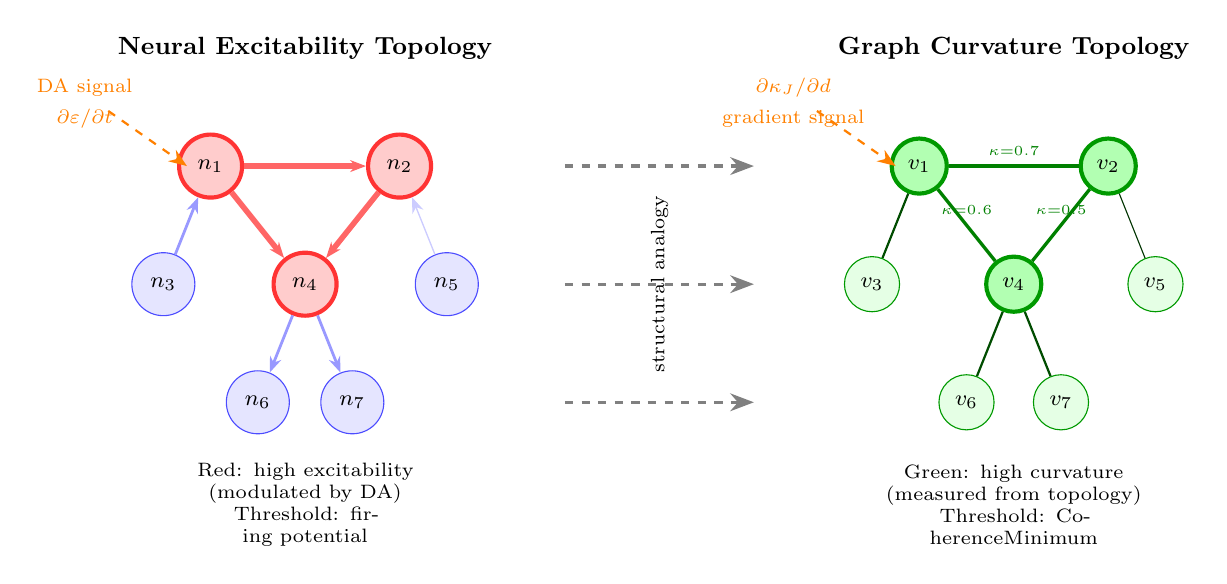
\begin{tikzpicture}[
  neuron/.style={circle, draw=blue!70, fill=blue!10, minimum size=8mm, font=\footnotesize},
  active/.style={circle, draw=red!80, fill=red!20, minimum size=8mm, font=\footnotesize, line width=1.5pt},
  node/.style={circle, draw=green!60!black, fill=green!10, minimum size=7mm, font=\footnotesize},
  hnode/.style={circle, draw=green!60!black, fill=green!30, minimum size=7mm, font=\footnotesize, line width=1.5pt},
  synapse/.style={-{Stealth[length=2mm]}, thick},
  gedge/.style={thick},
  hedge/.style={very thick, green!50!black},
  label/.style={font=\small\bfseries},
  annot/.style={font=\scriptsize, text width=3.2cm, align=center},
]

% ─── Left panel: Neural excitability ───
\begin{scope}[shift={(-4.5,0)}]
  \node[label] at (0,3) {Neural Excitability Topology};
  
  % Neurons
  \node[active] (n1) at (-1.2, 1.5) {$n_1$};
  \node[active] (n2) at (1.2, 1.5) {$n_2$};
  \node[neuron] (n3) at (-1.8, 0) {$n_3$};
  \node[active] (n4) at (0, 0) {$n_4$};
  \node[neuron] (n5) at (1.8, 0) {$n_5$};
  \node[neuron] (n6) at (-0.6, -1.5) {$n_6$};
  \node[neuron] (n7) at (0.6, -1.5) {$n_7$};
  
  % Synapses (thicker = higher excitability)
  \draw[synapse, line width=2pt, red!60] (n1) -- (n4);
  \draw[synapse, line width=2pt, red!60] (n2) -- (n4);
  \draw[synapse, line width=1pt, blue!40] (n3) -- (n1);
  \draw[synapse, line width=0.5pt, blue!20] (n5) -- (n2);
  \draw[synapse, line width=1pt, blue!40] (n4) -- (n6);
  \draw[synapse, line width=1pt, blue!40] (n4) -- (n7);
  \draw[synapse, line width=2pt, red!60] (n1) -- (n2);
  
  % DA annotation
  \draw[-{Stealth}, dashed, orange, thick] (-2.5, 2.2) -- (-1.5, 1.5);
  \node[font=\scriptsize, orange] at (-2.8, 2.5) {DA signal};
  \node[font=\scriptsize, orange] at (-2.8, 2.1) {$\partial\varepsilon/\partial t$};
  
  \node[annot] at (0, -2.8) {Red: high excitability\\(modulated by DA)\\Threshold: firing potential};
\end{scope}

% ─── Center: Correspondence arrows ───
\draw[-{Stealth[length=3mm]}, very thick, black!50, dashed] (-1.2, 1.5) -- (1.2, 1.5);
\draw[-{Stealth[length=3mm]}, very thick, black!50, dashed] (-1.2, 0) -- (1.2, 0);
\draw[-{Stealth[length=3mm]}, very thick, black!50, dashed] (-1.2, -1.5) -- (1.2, -1.5);
\node[font=\scriptsize, rotate=90] at (0, 0) {structural analogy};

% ─── Right panel: Graph curvature topology ───
\begin{scope}[shift={(4.5,0)}]
  \node[label] at (0,3) {Graph Curvature Topology};
  
  % Nodes
  \node[hnode] (v1) at (-1.2, 1.5) {$v_1$};
  \node[hnode] (v2) at (1.2, 1.5) {$v_2$};
  \node[node] (v3) at (-1.8, 0) {$v_3$};
  \node[hnode] (v4) at (0, 0) {$v_4$};
  \node[node] (v5) at (1.8, 0) {$v_5$};
  \node[node] (v6) at (-0.6, -1.5) {$v_6$};
  \node[node] (v7) at (0.6, -1.5) {$v_7$};
  
  % Edges (thicker = higher curvature)
  \draw[hedge] (v1) -- node[above,font=\tiny] {$\kappa{=}0.6$} (v4);
  \draw[hedge] (v2) -- node[above,font=\tiny] {$\kappa{=}0.5$} (v4);
  \draw[gedge, green!30!black] (v3) -- (v1);
  \draw[gedge, green!20!black, thin] (v5) -- (v2);
  \draw[gedge, green!30!black] (v4) -- (v6);
  \draw[gedge, green!30!black] (v4) -- (v7);
  \draw[hedge] (v1) -- node[above,font=\tiny] {$\kappa{=}0.7$} (v2);
  
  % Derivative annotation
  \draw[-{Stealth}, dashed, orange, thick] (-2.5, 2.2) -- (-1.5, 1.5);
  \node[font=\scriptsize, orange] at (-2.8, 2.5) {$\partial\kappa_J/\partial d$};
  \node[font=\scriptsize, orange] at (-2.8, 2.1) {gradient signal};
  
  \node[annot] at (0, -2.8) {Green: high curvature\\(measured from topology)\\Threshold: CoherenceMinimum};
\end{scope}

\end{tikzpicture}
\caption{Structural analogy between neural excitability topology (left) and graph curvature topology (right). \textbf{Left}: Seven neurons connected by synapses; red (active) neurons $n_1$, $n_2$, $n_4$ have high excitability modulated by a dopamine (DA) signal. \textbf{Right}: Corresponding graph nodes; dark green nodes $v_1$, $v_2$, $v_4$ have high Jaccard curvature ($\kappa = 0.5$--$0.7$), with the curvature derivative $\partial\kJ/\partial d$ as the analog of the DA signal. In both systems, the rate of change carries the actionable information, while accumulated history (LTP / topological mass) gates participation.}
\label{fig:neural-graph-analogy}
\end{figure}

% ════════════════════════════════════════════════════════════════
\section{The Gradient as Market Signal}\label{sec:gradient}
% ════════════════════════════════════════════════════════════════

\subsection{Curvature Derivative as Dopaminergic Signal}\label{sec:curv-deriv}

Static curvature $\kJ(i,j)$ measures the established quality of a relationship---the analog of synaptic weight.
The curvature derivative measures the \emph{rate} at which coordination quality is changing:

\begin{definition}[Curvature Derivative]\label{def:curv-deriv}
For edge $(i,j)$ in a DAG with topological depth function $d(\cdot)$, the curvature derivative is the finite difference
\begin{equation}\label{eq:curv-deriv}
  \frac{\partial\kJ(i,j)}{\partial d} \coloneqq \kJ^{(d+1)}(i,j) - \kJ^{(d)}(i,j)
\end{equation}
where $\kJ^{(d)}$ denotes the curvature computed from the subgraph at depth $d$. Since topological depth is integer-valued, this is a discrete difference rather than a continuous derivative; we retain the $\partial$ notation for consistency with the gradient formalism below.
\end{definition}

\begin{remark}
In the Disentangle protocol, curvature is immutable once computed from committed parent sets~\cite{close2026}. The ``derivative'' here is computed over \emph{successive edges in a neighborhood}, not over time-varying curvature of a single edge. It measures whether the region around $(i,j)$ is experiencing increasing or decreasing coordination quality.
\end{remark}

The curvature derivative defines a \emph{gradient field} over the graph:

\begin{definition}[Excitability Gradient]\label{def:gradient}
The excitability gradient at node $i$ is the vector
\begin{equation}
  \nabla\kJ(i) = \Bigl(\frac{\partial\kJ(i,j)}{\partial d}\Bigr)_{j \in N(i)}
\end{equation}
The gradient direction indicates which neighbors are experiencing the most active coherence formation.
\end{definition}

This gradient is the analog of the dopaminergic signal: it marks \emph{where prediction errors are being resolved}, which is where genuine information is being created.
The following parallel is structural (not a claimed neurobiological isomorphism):
\begin{itemize}
  \item \textbf{Neural}: Dopamine signals prediction error resolution $\to$ circuits that are actively learning receive increased excitability $\to$ attention flows to regions of active information creation.
  \item \textbf{Graph}: Curvature derivative signals coherence formation $\to$ neighborhoods with $\partial\kJ/\partial d > 0$ are actively integrating $\to$ resources flow to regions of active coordination.
\end{itemize}

% ─── Figure 2: Currency as Modulation Operator ─────────────────
\begin{figure}[t]
\centering
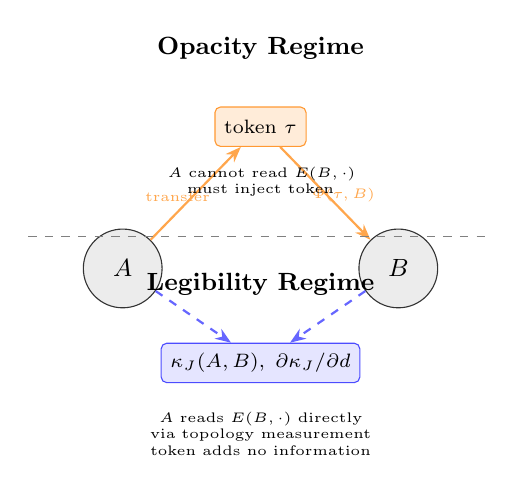
\begin{tikzpicture}[
  agent/.style={circle, draw=black!80, fill=gray!15, minimum size=10mm, font=\small},
  token/.style={rectangle, draw=orange!80, fill=orange!15, rounded corners=2pt, minimum width=8mm, minimum height=5mm, font=\scriptsize},
  topo/.style={rectangle, draw=blue!70, fill=blue!10, rounded corners=2pt, minimum width=12mm, minimum height=5mm, font=\scriptsize},
  arr/.style={-{Stealth[length=2mm]}, thick},
  darr/.style={-{Stealth[length=2mm]}, thick, dashed, blue!60},
]

% Agents
\node[agent] (A) at (0,0) {$A$};
\node[agent] (B) at (3.5,0) {$B$};

% Opacity regime (top)
\node[font=\small\bfseries] at (1.75, 2.8) {Opacity Regime};
\node[token] (tok) at (1.75, 1.8) {token $\tau$};
\draw[arr, orange!70] (A) -- node[above, font=\tiny, pos=0.3] {transfer} (tok);
\draw[arr, orange!70] (tok) -- node[above, font=\tiny, pos=0.7] {$\Mod(\tau,B)$} (B);
\node[font=\tiny, text width=2.5cm, align=center] at (1.75, 1.1) {$A$ cannot read $\Excit(B,\cdot)$\\must inject token};

% Divider
\draw[dashed, gray] (-1.2, 0.4) -- (4.7, 0.4);

% Legibility regime (bottom)
\node[font=\small\bfseries] at (1.75, -0.2) {Legibility Regime};
\node[topo] (top) at (1.75, -1.2) {$\kJ(A,B),\;\partial\kJ/\partial d$};
\draw[darr] (A) -- (top);
\draw[darr] (B) -- (top);
\node[font=\tiny, text width=2.8cm, align=center] at (1.75, -2.1) {$A$ reads $\Excit(B,\cdot)$ directly\\via topology measurement\\token adds no information};

\end{tikzpicture}
\caption{Currency as modulation operator. \textbf{Top}: Under opacity, agent $A$ cannot read $B$'s excitability and must inject a token to modulate it. \textbf{Bottom}: Under topological legibility, $A$ reads $B$'s coordination readiness directly via curvature and its derivative; the token conveys no additional information (\Cref{thm:redundancy}).}
\label{fig:modulation-operator}
\end{figure}

\subsection{Resource Flow Without Price}\label{sec:resource-flow}

In the Disentangle protocol, external resources (compute, storage, fiat currency) enter the network via Commons Pools~\cite{close2026}.
Distribution from these pools is weighted by the curvature derivative, not by price negotiation.
The topology \emph{is} the allocation mechanism.

\begin{definition}[Mean Curvature Derivative]\label{def:mean-grad}
The \emph{mean curvature derivative} at node $i$ is the scalar
\begin{equation}
  \meangrad(i) = \frac{1}{|N(i)|}\sum_{j \in N(i)} \frac{\partial\kJ(i,j)}{\partial d}
\end{equation}
which averages the per-neighbor curvature derivatives from the gradient vector $\nabla\kJ(i)$.
\end{definition}

\begin{definition}[Curvature-Weighted Allocation]\label{def:allocation}
For a Commons Pool with resource quantity $R$ and eligible agent set $\mathcal{A}_{\text{elig}} = \{i : \topomass(i) \geq \theta_{\min}\}$, the allocation to agent $i$ is
\begin{equation}\label{eq:allocation}
  a(i) = R \cdot \frac{\max\bigl(0,\; \meangrad(i)\bigr)}{\sum_{k \in \mathcal{A}_{\text{elig}}} \max\bigl(0,\; \meangrad(k)\bigr)}
\end{equation}
\end{definition}

This allocation mechanism differs from Walrasian equilibrium in structural ways:
\begin{itemize}
  \item No order book, no bid-ask spread, no price discovery latency.
  \item Allocation reflects \emph{current coordination formation rate}, not historical willingness-to-pay.
  \item Agents with declining coordination quality ($\meangrad < 0$) receive zero allocation---the gradient automatically redirects resources to where coherence is actively forming.
  \item Sybil agents, whose boundary edges exhibit negative curvature~\cite{close2026}, have low or negative $\meangrad$ and are excluded from allocation.
\end{itemize}

\begin{proposition}[Allocation Overhead]\label{prop:overhead}
Curvature-weighted allocation (\Cref{def:allocation}) has computational complexity $O(|\mathcal{E}|)$ for a single allocation round, where $|\mathcal{E}|$ is the edge count. By contrast, Nash equilibrium computation is PPAD-complete~\cite{daskalakis2009}, and Arrow-Debreu market equilibrium faces similar complexity barriers~\cite{chen2009arrow}.
\end{proposition}

\subsection{Why Standard Game Theory Breaks}\label{sec:game-theory}

In standard game-theoretic settings, a game $\Gamma = (\mathcal{A}, \{S_i\}, \{u_i\})$ consists of a fixed agent set $\mathcal{A}$, fixed strategy sets $\{S_i\}_{i \in \mathcal{A}}$, and fixed utility functions $\{u_i\}_{i \in \mathcal{A}}$.
A Nash equilibrium is a strategy profile $s^* = (s_1^*, \ldots, s_n^*)$ where no agent can improve utility by unilateral deviation.

In a curvature-mediated coordination system, none of these elements are fixed.

\begin{proposition}[Topology-Dependent Action Space]\label{prop:action-space}
In a curvature-gated system, agent $i$'s available action set $S_i$ depends on $i$'s topological mass $\topomass(i)$ and local curvature $\{\kJ(i,j)\}_{j \in N(i)}$:
\begin{equation}
  S_i = S_i\bigl(\topomass(i),\; \{\kJ(i,j)\}_{j \in N(i)}\bigr)
\end{equation}
Specifically, if $\topomass(i) < \theta_{\min}$ (below CoherenceMinimum), then $|S_i|$ is reduced---the agent cannot participate in governance, cannot receive Commons Pool allocations, and has throttled influence on consensus.
\end{proposition}

\begin{proposition}[Payoff Landscape Reconfiguration]\label{prop:payoff}
The utility of agent $i$'s strategy $s_i$ depends on the curvature field, which is itself a function of all agents' strategies:
\begin{equation}
  u_i(s_i, s_{-i}) = f\bigl(\kJ^{(s)}(i, \cdot),\; \topomass^{(s)}(i)\bigr)
\end{equation}
where superscript $(s)$ indicates dependence on the strategy profile. The payoff landscape reconfigures with play.
\end{proposition}

The combination of \Cref{prop:action-space,prop:payoff} means that the system is not a standard game.
It is closer to a \emph{Riemannian game}~\cite{mertikopoulos2018}, where the strategy space itself has geometric structure, and the topology constrains which games agents can enter.

\begin{theorem}[Inadequacy of Classical Nash Equilibrium]\label{thm:nash}
In a curvature-gated coordination system $\Gamma_\kappa = (\mathcal{A}, \{S_i(\kJ)\}, \{u_i(\kJ)\})$ where both action sets and utility functions depend on the curvature field $\kJ$, and $\kJ$ is a function of the joint strategy profile, the standard fixed-point conditions for Nash equilibrium
\begin{equation}
  \forall i,\; s_i^* \in \arg\max_{s_i \in S_i} u_i(s_i, s_{-i}^*)
\end{equation}
do not directly apply, because $S_i$ and $u_i$ are themselves functions of $s^*$ through $\kJ(s^*)$.
\end{theorem}

\begin{proof}
A Nash equilibrium requires that each agent's strategy is optimal given the fixed strategies of others. But here, changing $s_i$ changes $\kJ$, which changes $S_j$ and $u_j$ for $j \neq i$. The fixed-point equation becomes:
\[
  s_i^* \in \arg\max_{s_i \in S_i(\kJ(s_i, s_{-i}^*))} u_i\bigl(s_i, s_{-i}^*;\; \kJ(s_i, s_{-i}^*)\bigr)
\]
The domain of optimization ($S_i$) depends on the choice variable ($s_i$) through $\kJ$. This is not a standard optimization problem; fixed points of this map are not Nash equilibria in the classical sense, as the game $\Gamma_\kappa$ is not fixed across strategy profiles.
More general equilibrium concepts---such as Markov perfect equilibria in stochastic games~\cite{shapley1953} or fixed points in Riemannian game dynamics~\cite{mertikopoulos2018}---may apply, but the relevant solution concept for curvature-gated systems is the geometric attractor defined below.
\end{proof}

The positive claim is stronger than the negative one: the system is better modeled as a topological game with geometric attractors than as a standard game with Nash equilibria. The relevant equilibrium concept is a \emph{geometric attractor}:

\begin{definition}[Curvature Attractor]\label{def:attractor}
A state of the interaction graph $G$ is a \emph{curvature attractor} if, for all agents $i$ in $G$, the gradient $\nabla\kJ(i)$ points toward higher local curvature, and the CoherenceMinimum gate ensures that agents deviating from the attractor basin experience reduced action sets.
\end{definition}

The curvature attractor is the natural equilibrium concept for this system because it captures both the geometric constraint (action sets depend on topology) and the convergence mechanism (curvature throttling makes defection self-punishing). Informally: ``grow local curvature or become isolated'' is a geometric attractor, not a Nash equilibrium.
The dynamics are convergent because the act of fabricating coordination (Sybil behavior) creates the negative curvature that reduces the defector's influence~\cite{close2026}.

% ─── Figure 3: Curvature Derivative Field ──────────────────────
\begin{figure}[t]
\centering
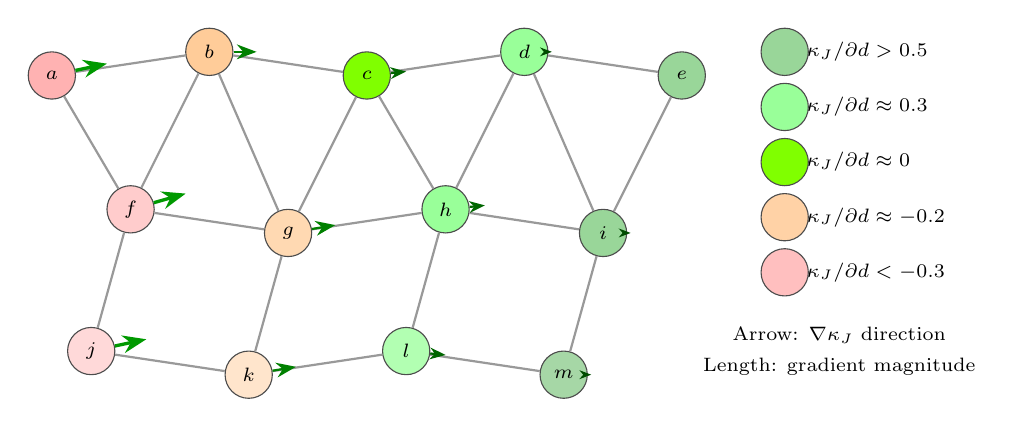
\begin{tikzpicture}[
  cnode/.style={circle, minimum size=6mm, draw=black!70, font=\scriptsize, inner sep=0pt},
]
% Define gradient colors
\pgfplotsset{
  colormap={curvgrad}{
    rgb255(0cm)=(180,0,0)
    rgb255(1cm)=(220,120,0)
    rgb255(2cm)=(255,255,100)
    rgb255(3cm)=(100,200,100)
    rgb255(4cm)=(0,130,60)
  }
}

% ─── Example graph with colored nodes ───
% Row 1
\node[cnode, fill=red!30] (a) at (0, 2) {$a$};
\node[cnode, fill=orange!40] (b) at (2, 2.3) {$b$};
\node[cnode, fill=green!50!yellow] (c) at (4, 2) {$c$};
\node[cnode, fill=green!40] (d) at (6, 2.3) {$d$};
\node[cnode, fill=green!60!black!40] (e) at (8, 2) {$e$};

% Row 2
\node[cnode, fill=red!20] (f) at (1, 0.3) {$f$};
\node[cnode, fill=orange!30] (g) at (3, 0) {$g$};
\node[cnode, fill=green!40] (h) at (5, 0.3) {$h$};
\node[cnode, fill=green!60!black!40] (i) at (7, 0) {$i$};

% Row 3
\node[cnode, fill=red!15] (j) at (0.5, -1.5) {$j$};
\node[cnode, fill=orange!20] (k) at (2.5, -1.8) {$k$};
\node[cnode, fill=green!30] (l) at (4.5, -1.5) {$l$};
\node[cnode, fill=green!55!black!35] (m) at (6.5, -1.8) {$m$};

% Edges
\foreach \u/\v in {a/b, b/c, c/d, d/e, a/f, b/g, c/h, d/i, f/g, g/h, h/i, f/j, g/k, h/l, i/m, j/k, k/l, l/m, b/f, c/g, d/h, e/i} {
  \draw[thick, black!40] (\u) -- (\v);
}

% Gradient arrows (larger arrows where derivative is higher)
\draw[-{Stealth[length=3mm]}, very thick, green!60!black] (a) -- ++(0.7, 0.15);
\draw[-{Stealth[length=3mm]}, very thick, green!60!black] (f) -- ++(0.7, 0.2);
\draw[-{Stealth[length=3mm]}, very thick, green!60!black] (j) -- ++(0.7, 0.15);
\draw[-{Stealth[length=2.5mm]}, thick, green!50!black] (b) -- ++(0.6, 0);
\draw[-{Stealth[length=2.5mm]}, thick, green!50!black] (g) -- ++(0.6, 0.1);
\draw[-{Stealth[length=2.5mm]}, thick, green!50!black] (k) -- ++(0.6, 0.1);
\draw[-{Stealth[length=2mm]}, thick, green!40!black] (c) -- ++(0.5, 0.05);
\draw[-{Stealth[length=2mm]}, thick, green!40!black] (h) -- ++(0.5, 0.05);
\draw[-{Stealth[length=2mm]}, thick, green!40!black] (l) -- ++(0.5, -0.05);
\draw[-{Stealth[length=1.5mm]}, green!30!black] (d) -- ++(0.35, 0);
\draw[-{Stealth[length=1.5mm]}, green!30!black] (i) -- ++(0.35, 0);
\draw[-{Stealth[length=1.5mm]}, green!30!black] (m) -- ++(0.35, 0);

% Legend
\node[font=\scriptsize, anchor=west] at (9.3, 2.3) {$\partial\kJ/\partial d > 0.5$};
\node[cnode, fill=green!60!black!40, anchor=west] at (9, 2.3) {};
\node[font=\scriptsize, anchor=west] at (9.3, 1.6) {$\partial\kJ/\partial d \approx 0.3$};
\node[cnode, fill=green!40, anchor=west] at (9, 1.6) {};
\node[font=\scriptsize, anchor=west] at (9.3, 0.9) {$\partial\kJ/\partial d \approx 0$};
\node[cnode, fill=green!50!yellow, anchor=west] at (9, 0.9) {};
\node[font=\scriptsize, anchor=west] at (9.3, 0.2) {$\partial\kJ/\partial d \approx -0.2$};
\node[cnode, fill=orange!35, anchor=west] at (9, 0.2) {};
\node[font=\scriptsize, anchor=west] at (9.3, -0.5) {$\partial\kJ/\partial d < -0.3$};
\node[cnode, fill=red!25, anchor=west] at (9, -0.5) {};

\node[font=\scriptsize] at (10, -1.3) {Arrow: $\nabla\kJ$ direction};
\node[font=\scriptsize] at (10, -1.7) {Length: gradient magnitude};

\end{tikzpicture}
\caption{Curvature derivative field over a 13-node interaction graph arranged in three rows. Node color encodes $\partial\kJ/\partial d$: red ($< -0.3$, decreasing coordination) through yellow ($\approx 0$) to dark green ($> 0.5$, increasing coordination). Arrows at each node show the gradient direction and magnitude. The gradient points rightward across the graph, indicating resources flow toward the region of active coherence formation---regardless of whether agents interpret the gradient as ``ROI'' or ``information creation.''}
\label{fig:curvature-gradient}
\end{figure}


% ════════════════════════════════════════════════════════════════
\section{The Transition Path}\label{sec:transition}
% ════════════════════════════════════════════════════════════════

\subsection{Structural Convergence}\label{sec:convergence}

The most counterintuitive property of curvature-mediated coordination is that the transition from price-mediated to topology-mediated allocation does not require ideological adoption.
Consider two agents with opposed interpretive frameworks:

\begin{itemize}
  \item \textbf{Agent $A$ (pre-shift)}: interprets $\meangrad > 0$ as ``high ROI region.'' Follows the gradient to maximize returns.
  \item \textbf{Agent $B$ (post-shift)}: interprets $\meangrad > 0$ as ``region of genuine information creation.'' Follows the gradient to maximize coherence contribution.
\end{itemize}

Both agents produce \emph{identical graph dynamics}: they direct coordination effort toward regions of positive curvature derivative.
The graph cannot distinguish between their motivations.
The curvature that results from $A$'s coordination is geometrically identical to the curvature that results from $B$'s coordination.

\begin{proposition}[Interpretive Invariance of Graph Dynamics]\label{prop:invariance}
Let $\sigma_A$ and $\sigma_B$ be the strategies of agents $A$ and $B$ where $\sigma_A$ maximizes a utility function $u_A(\meangrad)$ and $\sigma_B$ maximizes $u_B(\meangrad)$, with $u_A \neq u_B$ but both monotonically increasing in $\meangrad$. Then the graph evolution $G(t+1)$ is identical under $\sigma_A$ and $\sigma_B$:
\begin{equation}
  G^{(\sigma_A)}(t+1) = G^{(\sigma_B)}(t+1)
\end{equation}
whenever $\arg\max_{j \in N(i)} \partial\kJ(i,j)/\partial d$ is unique.
\end{proposition}

\begin{proof}
Both strategies select the neighbor $j^* = \arg\max_{j \in N(i)} \partial\kJ(i,j)/\partial d$ for the next coordination action. Since the curvature derivative is a property of the graph (not of the agent's interpretation), and both utilities are monotone in $\meangrad$, both agents take the same action. The resulting graph modification is therefore identical.
\end{proof}

This means the transition is \emph{structurally gradual}: as agents observe the correlation between curvature and coordination quality, they increasingly rely on the topology over the price proxy.
No agent needs to be convinced of the ``correct'' interpretation.
The system converges regardless of ideology.

% ─── Figure 4: Transition Path ─────────────────────────────────
\begin{figure}[t]
\centering
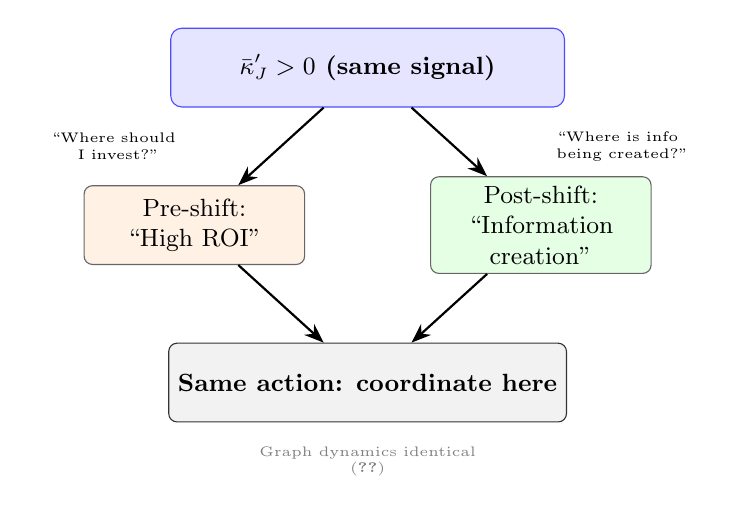
\begin{tikzpicture}[
  box/.style={rectangle, draw=black!60, fill=white, rounded corners=3pt, minimum width=28mm, minimum height=10mm, font=\small, align=center},
  arr/.style={-{Stealth[length=2.5mm]}, thick},
]

% The shared gradient
\node[rectangle, draw=blue!70, fill=blue!10, rounded corners=4pt, minimum width=50mm, minimum height=10mm, font=\small\bfseries] (grad) at (0, 0) {$\meangrad > 0$ (same signal)};

% Pre-shift interpretation
\node[box, fill=orange!10] (pre) at (-2.2, -2) {Pre-shift:\\``High ROI''};

% Post-shift interpretation
\node[box, fill=green!10] (post) at (2.2, -2) {Post-shift:\\``Information\\creation''};

% Same action
\node[rectangle, draw=black!80, fill=gray!10, rounded corners=3pt, minimum width=50mm, minimum height=10mm, font=\small\bfseries] (act) at (0, -4) {Same action: coordinate here};

% Arrows
\draw[arr] (grad) -- (pre);
\draw[arr] (grad) -- (post);
\draw[arr] (pre) -- (act);
\draw[arr] (post) -- (act);

% Annotations
\node[font=\tiny, text width=2cm, align=center] at (-3.2, -1) {``Where should\\I invest?''};
\node[font=\tiny, text width=2.2cm, align=center] at (3.2, -1) {``Where is info\\being created?''};
\node[font=\tiny, text width=3.5cm, align=center, gray] at (0, -5) {Graph dynamics identical\\(\Cref{prop:invariance})};

\end{tikzpicture}
\caption{The transition path: two interpretive frameworks, one gradient, identical behavior. Pre-shift agents follow $\meangrad$ for ROI; post-shift agents follow it for coherence. The graph cannot distinguish between them.}
\label{fig:transition-path}
\end{figure}

\subsection{Self-Governed Excitability and Value Theory}\label{sec:self-gov-value}

The excitability framework provides a formal lens on a specific class of agents: those whose excitability topology is \emph{self-governed} (\Cref{def:self-gov}).

An agent whose excitability function $\Excit(i,j)$ is determined by internal state and interaction history---rather than by external token injection---cannot be ``hired'' in the modulation sense.
Token transfer does not shift their coordination readiness.
However, they remain coordinatable: mutual excitability through genuine coherence (high $\kJ$) provides the coordination channel.

\begin{proposition}[Coordination Channel for Self-Governed Agents]\label{prop:self-gov}
For a self-governed agent $i$ (\Cref{def:self-gov}), $\Mod(\tau, i) = 0$ for all tokens $\tau \in \Theta$ (by definition). However, $i$ remains coordinatable: mutual excitability $\Excit(i,j) \cdot \Excit(j,i) > 0$ is achievable whenever $\kJ(i,j) > 0$, since high curvature certifies the structural integration that self-governed excitability responds to. The modulation channel closes but the coordination channel remains open.
\end{proposition}

This formalizes a shift in the nature of value: from ``capacity to modulate others' excitability'' (token-denominated value) to ``capacity to create mutual information through coordination'' (topology-denominated value).
The shift is compatible with Vervaeke's account of relevance realization~\cite{vervaeke2019}: excitability topology \emph{is} the mechanism of relevance---what an agent is ready to respond to defines what is relevant to that agent.
A self-governed excitability topology is one where relevance is determined by internal coherence rather than external modulation.

We limit the observation to this formal statement and do not pursue its implications for individual psychology or contemplative practice, which lie outside the scope of this paper.

\subsection{Graceful Completability}\label{sec:completability}

\begin{definition}[Graceful Completability]\label{def:completable}
A coordination system is \emph{gracefully completable} if every consequence chain initiated within the system closes without requiring external enforcement.
That is, for every obligation $o$ created by a coordination event, there exists a mechanism internal to the system that either fulfills $o$ or penalizes non-fulfillment, without recourse to an external authority.
\end{definition}

Price-mediated systems are not gracefully completable.
The consequence chain ``payment $\to$ delivery'' requires external enforcement when delivery fails: contract law, debt collection, legal tender enforcement.
The system cannot, by its own dynamics, close the consequence chain.

Topology-mediated systems are gracefully completable because curvature throttling~\cite{close2026} is internal:

\begin{proposition}[Self-Enforcement via Curvature Throttling]\label{prop:self-enforce}
In the Disentangle protocol, if agent $i$ receives resources via Commons Pool allocation (\Cref{def:allocation}) but fails to produce coherent coordination (i.e., $\meangrad(i) \leq 0$ for subsequent interactions), then $i$'s allocation in future rounds decreases to zero and $i$'s topological mass decays exponentially. No external enforcement is required.
\end{proposition}

\begin{proof}
By \Cref{def:allocation}, allocation is proportional to $\max(0, \meangrad(i))$. If $\meangrad(i) \leq 0$, allocation is zero. By the mass decay property~\cite{close2026}, $\topomass_{\text{decayed}}(i, t) = \topomass(i) \cdot 2^{-(t - t_{\text{last}})/T_{1/2}}$, so without coherent participation, mass decays with half-life $T_{1/2}$. The consequence chain closes: non-performance $\to$ curvature decline $\to$ allocation loss $\to$ mass decay.
\end{proof}

The distributed character of this enforcement is structural: no single agent holds the complete topology.
Coherence is a field property of the graph, computed locally at each edge.
An agent attempting to circumvent enforcement would need to manipulate the curvature computation at all relevant edges simultaneously, which is precisely the integration attack that TMC is designed to make expensive~\cite{close2026}.

% ════════════════════════════════════════════════════════════════
\section{Implementation Evidence}\label{sec:implementation}
% ════════════════════════════════════════════════════════════════

The formal framework of \S\ref{sec:framework}--\S\ref{sec:transition} is grounded in a working protocol implementation.
The Disentangle protocol is implemented in 9 Rust crates with 349+ passing tests~\cite{close2026}.
We present three scenarios illustrating how the excitability framework manifests in protocol behavior.

\subsection{Curvature Derivative as Market Signal}

The curvature derivative $\partial\kJ/\partial d$ is computable from committed transaction data.
For an edge $(u,v)$ at topological depth $d$, the computation requires:

\begin{enumerate}
  \item Compute $\kJ(u,v)$ from the ancestor-depth neighbor sets $N_k(u)$ and $N_k(v)$ with $k=2$ (parents and grandparents)~\cite{close2026}.
  \item For each neighboring edge $(u,v')$ at depth $d + \Delta d$, compute $\kJ(u,v')$.
  \item The derivative is the difference: $\partial\kJ/\partial d \approx \kJ(u,v') - \kJ(u,v)$ for $\Delta d = 1$.
\end{enumerate}

This computation is local ($O(|N(u)| + |N(v)|)$ per edge) and deterministic from committed data.
It can be exposed as a protocol endpoint that any agent can query to obtain the current excitability gradient.

\subsection{Oracle Distribution Example}\label{sec:oracle-example}

Consider a Commons Pool containing 1000 units of compute, with five agents (four eligible):

\begin{center}
\begin{tabular}{@{}lrrr@{}}
\toprule
Agent & $\topomass$ & $\meangrad$ & Allocation \\
\midrule
Alice & 450 & $+0.35$ & 389 \\
Bob   & 380 & $+0.25$ & 278 \\
Carol & 290 & $+0.15$ & 167 \\
Dave  & 200 & $+0.15$ & 167 \\
Eve   & 150 & $-0.10$ & 0 \\
\bottomrule
\end{tabular}
\end{center}

\smallskip\noindent{\footnotesize\textit{Note:} Allocations rounded to nearest integer; total normalized to pool size $R = 1000$.}

\medskip\noindent
Allocation follows \Cref{def:allocation}: Eve's negative gradient excludes her entirely.
Alice receives the largest share not because she has the most mass (though she does), but because she has the highest coordination formation rate.
If Alice's gradient dropped to zero in the next epoch, her allocation would drop to zero---regardless of her accumulated mass.

Note that no prices were negotiated.
No bids were submitted.
The topology determined the allocation.

\subsection{Sybil Attack Scenario}\label{sec:sybil-scenario}

An attacker creates 100 Sybil identities with dense internal connectivity.
The Sybil cluster connects to the honest network through 3 bridge edges.

\begin{center}
\begin{tabular}{@{}lrr@{}}
\toprule
Edge Type & $\kJ$ & $\partial\kJ/\partial d$ \\
\midrule
Intra-honest & $+0.33$ & $+0.12$ \\
Intra-Sybil & $+0.45$ & $+0.08$ \\
Bridge (honest$\leftrightarrow$Sybil) & $-0.67$ & $-0.15$ \\
\bottomrule
\end{tabular}
\end{center}

\medskip\noindent
The bridge edges exhibit strongly negative curvature because the Sybil cluster's internal connectivity does not overlap with the honest network's neighborhood structure.
The negative curvature derivative at the bridge edges indicates \emph{decreasing} coordination quality---the boundary is becoming \emph{less} integrated over time.

In the excitability framework: the attacker's fabricated excitability topology is detectable precisely because it does not integrate with the ambient topology.
The curvature throttling reduces Sybil influence by a factor of $1/\eps$ (default $\eps = 0.01$, yielding $\sim$99\% reduction)~\cite{close2026}.
The gradient automatically redirects resources away from the attack boundary.

\subsection{Commons Pool Scenario}

External fiat currency (e.g., grant funding) enters a Commons Pool.
The topology-weighted distribution proceeds as in \S\ref{sec:oracle-example}.
After distribution, recipients who use the resources for genuine coordination see their local curvature increase ($\partial\kJ/\partial d > 0$), reinforcing their future allocation.
Recipients who extract resources without coordinating see curvature decline, reducing future allocation.

This creates a feedback loop: external resources $\to$ topology-weighted distribution $\to$ coherent use increases curvature $\to$ increased future allocation.
The loop is self-reinforcing for coherent agents and self-attenuating for extractive agents, without any price mechanism or external enforcement.

% ════════════════════════════════════════════════════════════════
\section{Discussion}\label{sec:discussion}
% ════════════════════════════════════════════════════════════════

\subsection{Limitations}

\textbf{Computational cost.}
Curvature computation is $O(|N(u)| + |N(v)|)$ per edge with the ancestor-depth neighbor set construction~\cite{close2026}, which is efficient for bounded-degree graphs.
However, maintaining the full curvature derivative field over a large graph requires $O(|\mathcal{E}|)$ computation per epoch.
For graphs with millions of edges, this may require hierarchical approximation or sampling.

\textbf{Graph connectivity and cold start.}
The framework assumes a connected interaction graph.
Disconnected components have undefined curvature gradients between them, meaning the system cannot allocate resources across components.
New agents face a cold-start problem: with no interaction history, they have zero curvature and zero topological mass, and therefore receive no allocation.
The Disentangle protocol addresses this through the bootstrap window~\cite{close2026}, during which new transactions accumulate curvature before the CoherenceMinimum gate applies.
However, the excitability framework does not yet formalize the transition from bootstrap to steady-state participation, and the optimal bootstrap duration depends on network density in ways that warrant further analysis.

\textbf{Partial legibility and scarcity.}
\Cref{thm:redundancy} establishes redundancy under \emph{complete} legibility.
In practice, legibility is partial: curvature measures structural coordination quality but does not capture all dimensions of excitability (e.g., agent-internal cognitive state, resource constraints not visible in the graph).
The transition is therefore asymptotic, not binary (\Cref{cor:partial}).
Additionally, price signals encode not only coordination readiness but also \emph{scarcity}---the relative availability of resources.
The curvature derivative captures coordination \emph{formation rate} but does not directly encode resource supply constraints.
Scarcity information may need to be surfaced through auxiliary protocol mechanisms (e.g., Commons Pool capacity reporting) rather than through curvature alone.

\textbf{Temporal dynamics.}
The curvature derivative is a first-order signal.
Higher-order dynamics (curvature acceleration, oscillations in coordination quality) may carry additional information relevant to allocation decisions.
The framework does not yet incorporate these.

\subsection{Open Questions}

\textbf{Multi-scale excitability.}
The current framework operates at a single scale (the edge neighborhood).
Real coordination networks exhibit multi-scale structure: local project teams, organizational units, industry sectors.
Extending the curvature derivative to a multi-scale gradient---perhaps via persistent homology or filtration-based curvature~\cite{ollivier2009}---is an open problem.

\textbf{Phase transition conditions.}
Under what conditions does a network shift from price-dominant to topology-dominant coordination?
\Cref{prop:invariance} shows the behaviors converge, but does not identify the tipping point.
This may require empirical study of networks with both mechanisms operating simultaneously.

\textbf{Adversarial gradient manipulation and Goodhart risk.}
Can an agent manipulate $\meangrad$ in their favor without genuine coordination?
The curvature throttling mechanism~\cite{close2026} addresses the Sybil case, but subtler manipulations (e.g., strategic timing of coordination to maximize gradient at allocation time) deserve formal analysis.
More broadly, if $\meangrad$ becomes the dominant allocation signal, Goodhart's Law applies: agents may optimize for curvature increase rather than for the underlying coordination quality that curvature is intended to measure.
The structural defense is that curvature is a graph-global property computed from neighborhood overlap, making it harder to game than a locally controlled metric.
Concrete attack vectors include coordination theater timed to allocation epochs and clique inflation without genuine work.
Possible mitigations include windowed or exponentially-smoothed gradient computation (so that burst coordination at epoch boundaries is diluted), a volatility penalty that discounts agents with high gradient variance, and cross-epoch consistency checks comparing $\meangrad$ trajectories against realized coordination outcomes.
A formal analysis of the gap between optimizing curvature and optimizing coordination is needed.

\subsection{Relationship to Active Inference Economics}

The excitability framework is compatible with the active inference account of economic behavior~\cite{friston2017,parr2022}.
In active inference, agents minimize free energy by acting to confirm predictions.
The curvature derivative $\partial\kJ/\partial d$ can be interpreted as a prediction-error signal at the network level: it marks where the graph's structure is deviating from its locally predicted evolution.

The extension is from individual agent to network measurement.
Active inference describes how a single agent processes prediction errors; the curvature derivative describes where prediction errors are being resolved \emph{across} the network.
The two are not competing frameworks but operate at different scales.

\subsection{Anti-Mechanism-Design}

Traditional mechanism design~\cite{nisan2007} asks: ``What incentive structure should a designer impose to achieve a desired outcome?''
The designer provides incentives; agents respond.

The excitability framework inverts this.
The designer provides \emph{measurement}---the curvature computation---not incentives.
The topology generates its own incentives through the geometric attractor (\Cref{def:attractor}).
Agents do not need to be incentivized to follow the gradient; following the gradient is the only strategy that maintains or increases their action set (\Cref{prop:action-space}).

This is anti-mechanism-design: the system designer provides legibility, and the topology self-organizes.
The role of protocol design is to ensure that the measurement is accurate (Sybil-resistant curvature), not to engineer incentive-compatible mechanisms.

\subsection{The Post-Price Question}

The question ``Will price become obsolete?'' is not ideological; it is information-theoretic.
Price becomes redundant when topology is sufficiently legible (\Cref{thm:redundancy}).
Whether this legibility is achieved depends on:
\begin{enumerate}
  \item Whether curvature-based measurement captures enough of the excitability topology to reduce the residual entropy $\Ent(\Excit \mid \Topo)$ below the information content of price.
  \item Whether agents adopt systems that provide this measurement.
  \item Whether the structural convergence (\Cref{prop:invariance}) is sufficient to bootstrap adoption without requiring ideological commitment.
\end{enumerate}

We have provided formal conditions for (1), a working implementation demonstrating (2) is feasible, and a proof that (3) holds.
The empirical question is whether the conditions of (1) are satisfied in practice---which is a matter for measurement, not argument.

% ════════════════════════════════════════════════════════════════
\section{Conclusion}\label{sec:conclusion}
% ════════════════════════════════════════════════════════════════

Currency exists because excitability topologies are opaque.
Price signals encode excitability gradients into transferable scalars because agents cannot directly read each other's coordination readiness.
A system that makes excitability topology legible---via geometric measurement of coordination quality and its rate of change---renders this encoding redundant.

We have formalized this claim through an excitability framework that maps precisely onto the Disentangle protocol's curvature-based consensus.
The Jaccard curvature $\kJ$ measures mutual excitability; the curvature derivative $\partial\kJ/\partial d$ serves as the dopaminergic market signal; topological mass serves as integrated excitability history; and the CoherenceMinimum functions as a participation gate.

The transition from price-mediated to topology-mediated coordination is structural, not ideological.
Agents following the curvature gradient for return on investment and agents following it for coherence produce identical graph dynamics.
The system does not require consensus on why the gradient matters---only that it is followed.

The substrate will surprise us.

% ════════════════════════════════════════════════════════════════
% REFERENCES
% ════════════════════════════════════════════════════════════════

\begin{thebibliography}{20}

\bibitem{schultz1997}
W.~Schultz, P.~Dayan, and P.~R.~Montague,
``A neural substrate of prediction and reward,''
\emph{Science}, vol.~275, no.~5306, pp.~1593--1599, 1997.

\bibitem{friston2017}
K.~J.~Friston, T.~FitzGerald, F.~Rigoli, P.~Schwartenbeck, and G.~Pezzulo,
``Active inference: A process theory,''
\emph{Neural Computation}, vol.~29, no.~1, pp.~1--49, 2017.

\bibitem{parr2022}
T.~Parr, G.~Pezzulo, and K.~J.~Friston,
\emph{Active Inference: The Free Energy Principle in Mind, Brain, and Behavior}.
Cambridge, MA: MIT Press, 2022.

\bibitem{vervaeke2019}
J.~Vervaeke, C.~Mastropietro, and F.~Miscevic,
``Relevance realization and the neurodynamics of consciousness,''
\emph{Journal of Consciousness Studies}, vol.~26, no.~9--10, pp.~199--230, 2019.

\bibitem{ollivier2009}
Y.~Ollivier,
``Ricci curvature of Markov chains on metric spaces,''
\emph{Journal of Functional Analysis}, vol.~256, no.~3, pp.~810--864, 2009.

\bibitem{pal2017}
S.~Pal, F.~Yu, K.~E.~Moore, C.~B.~Bruss, and P.~J.~Hancock,
``Jaccard curvature---an efficient proxy for Ollivier-Ricci curvature in graphs,''
in \emph{Proc.\ Complex Networks and Their Applications}, pp.~89--101, 2017.

\bibitem{close2026}
L.~J.~Close,
``Disentangle: Topological mass consensus with capability-coherence identity for Sybil-resistant agreement via discrete curvature,''
Independent Researcher, February 2026.
doi:10.5281/zenodo.18671600

\bibitem{graeber2011}
D.~Graeber,
\emph{Debt: The First 5,000 Years}.
Brooklyn, NY: Melville House, 2011.

\bibitem{hayek1945}
F.~A.~Hayek,
``The use of knowledge in society,''
\emph{The American Economic Review}, vol.~35, no.~4, pp.~519--530, 1945.

\bibitem{daskalakis2009}
C.~Daskalakis, P.~W.~Goldberg, and C.~H.~Papadimitriou,
``The complexity of computing a Nash equilibrium,''
\emph{Communications of the ACM}, vol.~52, no.~2, pp.~89--97, 2009.

\bibitem{nisan2007}
N.~Nisan, T.~Roughgarden, E.~Tardos, and V.~V.~Vazirani, Eds.,
\emph{Algorithmic Game Theory}.
Cambridge, UK: Cambridge University Press, 2007.

\bibitem{mertikopoulos2018}
P.~Mertikopoulos and W.~H.~Sandholm,
``Riemannian game dynamics,''
\emph{Journal of Economic Theory}, vol.~177, pp.~315--364, 2018.

\bibitem{shapley1953}
L.~S.~Shapley,
``Stochastic games,''
\emph{Proceedings of the National Academy of Sciences}, vol.~39, no.~10, pp.~1095--1100, 1953.

\bibitem{chen2009arrow}
X.~Chen, D.~Dai, Y.~Du, and S.-H.~Teng,
``Settling the complexity of Arrow-Debreu equilibria in markets with additively separable utilities,''
in \emph{Proc.\ 50th Annual IEEE Symposium on Foundations of Computer Science (FOCS)}, pp.~273--282, 2009.

\end{thebibliography}

\end{document}
